
    \section{Štirikotnik in pravilni $n$-kotnik}

                 
                \textbf{Štirikotnike} delimo glede na število parov vzporednih stranic v tri skupine:
                \begin{itemize}
                    \item \textbf{paralelograme}, ki imajo dva para vzporednih stranic;
                    \item \textbf{trapeze}, ki imajo en par vzporednih stranic;
                    \item \textbf{trapezoide}, ki nimajo nobenega para vzporednih stranic.
                \end{itemize}
            

            
                Vsak štirikotnik ima dve diagonali. 

                Diagonala $e$ povezuje oglišči $A$ in $C$, diagonala $f$ pa oglišči $B$ in $D$.
            

            \begin{izrek}
                Vsota notranjih kotov štirikotnika je $360^\circ$. 
                $$\alpha + \beta + \gamma + \delta = 360^\circ$$
            \end{izrek}
        


        
            \subsection*{Paralelogram}
            
            
                \begin{figure}[H]
                    \centering
                    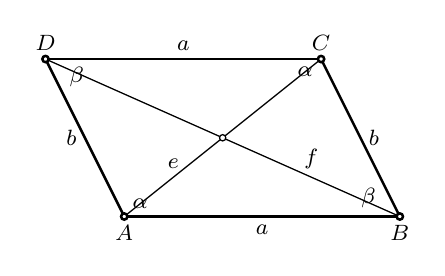
\begin{tikzpicture}
                    % \clip (0,0) rectangle (14.000000,10.000000);
                    {\footnotesize

                    % Marking point a
                    \draw (4.250000,1.500000) node [anchor=north] { $a$ };%

                    % Marking point a
                    \draw (3.250000,3.500000) node [anchor=south] { $a$ };%

                    % Marking point b
                    \draw (5.500000,2.500000) node [anchor=west] { $b$ };%

                    % Marking point b
                    \draw (2.000000,2.500000) node [anchor=east] { $b$ };%

                    % Drawing segment A C
                    \draw [line width=0.016cm] (2.531235,1.524988) -- (3.718765,2.475012);%
                    \draw [line width=0.016cm] (3.781235,2.524988) -- (4.968765,3.475012);%

                    % Drawing segment B D
                    \draw [line width=0.016cm] (5.963448,1.516246) -- (3.786552,2.483754);%
                    \draw [line width=0.016cm] (3.713448,2.516246) -- (1.536552,3.483754);%

                    % Marking point S by circle
                    \draw [line width=0.016cm] (3.750000,2.500000) circle (0.040000);%

                    % Marking point e
                    \draw (3.125000,2.000000) node [anchor=south] { $e$ };%

                    % Marking point f
                    \draw (4.875000,2.000000) node [anchor=south] { $f$ };%

                    % Marking point \alpha
                    \draw (2.500000,1.500000) node [anchor=south west] { $\alpha$ };%

                    % Marking point \beta
                    \draw (5.800000,1.500000) node [anchor=south east] { $\beta$ };%

                    % Marking point \alpha
                    \draw (5.000000,3.500000) node [anchor=north east] { $\alpha$ };%

                    % Marking point \beta
                    \draw (1.700000,3.500000) node [anchor=north west] { $\beta$ };%

                    % Drawing segment A B
                    \draw [line width=0.032cm] (2.540000,1.500000) -- (5.960000,1.500000);%

                    % Drawing segment B C
                    \draw [line width=0.032cm] (5.982111,1.535777) -- (5.017889,3.464223);%

                    % Drawing segment C D
                    \draw [line width=0.032cm] (4.960000,3.500000) -- (1.540000,3.500000);%

                    % Drawing segment D A
                    \draw [line width=0.032cm] (1.517889,3.464223) -- (2.482111,1.535777);%

                    % Marking point A by circle
                    \draw [line width=0.032cm] (2.500000,1.500000) circle (0.040000);%
                    \draw (2.500000,1.500000) node [anchor=north] { $A$ };%

                    % Marking point B by circle
                    \draw [line width=0.032cm] (6.000000,1.500000) circle (0.040000);%
                    \draw (6.000000,1.500000) node [anchor=north] { $B$ };%

                    % Marking point C by circle
                    \draw [line width=0.032cm] (5.000000,3.500000) circle (0.040000);%
                    \draw (5.000000,3.500000) node [anchor=south] { $C$ };%

                    % Marking point D by circle
                    \draw [line width=0.032cm] (1.500000,3.500000) circle (0.040000);%
                    \draw (1.500000,3.500000) node [anchor=south] { $D$ };%
                    }
                    \end{tikzpicture}

                \end{figure}
            

            \begin{izrek}
                Naslednje trditve so enakovredne in karakterizirajo paralelogram:
                \begin{enumerate}
                    \item Poljubni nasprotni stranici sta skladni ($|AB|=|CD|=a$ in $|AD|=|BC|=b$).
                    \item Diagionali se razpolavljata.
                    \item Poljubna sosednja kota sta suplementarna ($\alpha+\beta=180^\circ$).
                    \item Poljubna nasprotna kota sta skladna.
                \end{enumerate}
            \end{izrek}

            
                Višina paralelograma je razdalja med vzporednima stranicama.
            
        

        
            
                Paralelograme delimo na \textit{pravokotne} in \textit{poševnokotne} oziroma na \textit{enakostranične} in \textit{raznostranične}.
            

            \begin{definicija}
                \textbf{Pravokotnik} je pravokotni raznostranični paralelogram.

                \begin{figure}[H]
                    \centering
                    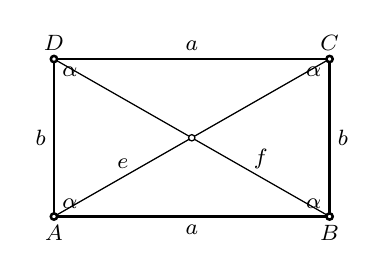
\begin{tikzpicture}
                    % \clip (0,0) rectangle (14.000000,10.000000);
                    {\footnotesize

                    % Marking point a
                    \draw (3.250000,1.500000) node [anchor=north] { $a$ };%

                    % Marking point a
                    \draw (3.250000,3.500000) node [anchor=south] { $a$ };%

                    % Marking point b
                    \draw (5.000000,2.500000) node [anchor=west] { $b$ };%

                    % Marking point b
                    \draw (1.500000,2.500000) node [anchor=east] { $b$ };%

                    % Drawing segment A C
                    \draw [line width=0.016cm] (1.534730,1.519846) -- (3.215270,2.480154);%
                    \draw [line width=0.016cm] (3.284730,2.519846) -- (4.965270,3.480154);%

                    % Drawing segment B D
                    \draw [line width=0.016cm] (4.965270,1.519846) -- (3.284730,2.480154);%
                    \draw [line width=0.016cm] (3.215270,2.519846) -- (1.534730,3.480154);%

                    % Marking point S by circle
                    \draw [line width=0.016cm] (3.250000,2.500000) circle (0.040000);%

                    % Marking point e
                    \draw (2.375000,2.000000) node [anchor=south] { $e$ };%

                    % Marking point f
                    \draw (4.125000,2.000000) node [anchor=south] { $f$ };%

                    % Marking point \alpha
                    \draw (1.500000,1.500000) node [anchor=south west] { $\alpha$ };%

                    % Marking point \beta
                    \draw (5.000000,1.500000) node [anchor=south east] { $\alpha$ };%

                    % Marking point \alpha
                    \draw (5.000000,3.500000) node [anchor=north east] { $\alpha$ };%

                    % Marking point \beta
                    \draw (1.500000,3.500000) node [anchor=north west] { $\alpha$ };%

                    % Drawing segment A B
                    \draw [line width=0.032cm] (1.540000,1.500000) -- (4.960000,1.500000);%

                    % Drawing segment B C
                    \draw [line width=0.032cm] (5.000000,1.540000) -- (5.000000,3.460000);%

                    % Drawing segment C D
                    \draw [line width=0.032cm] (4.960000,3.500000) -- (1.540000,3.500000);%

                    % Drawing segment D A
                    \draw [line width=0.032cm] (1.500000,3.460000) -- (1.500000,1.540000);%

                    % Marking point A by circle
                    \draw [line width=0.032cm] (1.500000,1.500000) circle (0.040000);%
                    \draw (1.500000,1.500000) node [anchor=north] { $A$ };%

                    % Marking point B by circle
                    \draw [line width=0.032cm] (5.000000,1.500000) circle (0.040000);%
                    \draw (5.000000,1.500000) node [anchor=north] { $B$ };%

                    % Marking point C by circle
                    \draw [line width=0.032cm] (5.000000,3.500000) circle (0.040000);%
                    \draw (5.000000,3.500000) node [anchor=south] { $C$ };%

                    % Marking point D by circle
                    \draw [line width=0.032cm] (1.500000,3.500000) circle (0.040000);%
                    \draw (1.500000,3.500000) node [anchor=south] { $D$ };%
                    }
                    \end{tikzpicture}
                \end{figure}
            \end{definicija}

            
                Diagonali v pravokotniku sta skladni ($e=f$) in se razpolavljata;
                vsi notranji koti so pravi ($\alpha=90^\circ$);
                višine so stranice same.
            


        


        
            \begin{definicija}
                \textbf{Kvadrat} je pravokotni enakostranični paralelogram.

                \begin{figure}[H]
                    \centering
                    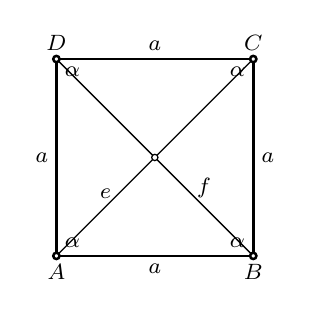
\begin{tikzpicture}
                    % \clip (0,0) rectangle (14.000000,10.000000);
                    {\footnotesize

                    % Marking point a
                    \draw (2.750000,1.500000) node [anchor=north] { $a$ };%

                    % Marking point a
                    \draw (2.750000,4.000000) node [anchor=south] { $a$ };%

                    % Marking point a
                    \draw (4.000000,2.750000) node [anchor=west] { $a$ };%

                    % Marking point a
                    \draw (1.500000,2.750000) node [anchor=east] { $a$ };%

                    % Drawing segment A C
                    \draw [line width=0.016cm] (1.528284,1.528284) -- (2.721716,2.721716);%
                    \draw [line width=0.016cm] (2.778284,2.778284) -- (3.971716,3.971716);%

                    % Drawing segment B D
                    \draw [line width=0.016cm] (3.971716,1.528284) -- (2.778284,2.721716);%
                    \draw [line width=0.016cm] (2.721716,2.778284) -- (1.528284,3.971716);%

                    % Marking point S by circle
                    \draw [line width=0.016cm] (2.750000,2.750000) circle (0.040000);%

                    % Marking point e
                    \draw (2.125000,2.125000) node [anchor=south] { $e$ };%

                    % Marking point f
                    \draw (3.375000,2.125000) node [anchor=south] { $f$ };%

                    % Marking point \alpha
                    \draw (1.500000,1.500000) node [anchor=south west] { $\alpha$ };%

                    % Marking point \alpha
                    \draw (4.000000,1.500000) node [anchor=south east] { $\alpha$ };%

                    % Marking point \alpha
                    \draw (4.000000,4.000000) node [anchor=north east] { $\alpha$ };%

                    % Marking point \alpha
                    \draw (1.500000,4.000000) node [anchor=north west] { $\alpha$ };%

                    % Drawing segment A B
                    \draw [line width=0.032cm] (1.540000,1.500000) -- (3.960000,1.500000);%

                    % Drawing segment B C
                    \draw [line width=0.032cm] (4.000000,1.540000) -- (4.000000,3.960000);%

                    % Drawing segment C D
                    \draw [line width=0.032cm] (3.960000,4.000000) -- (1.540000,4.000000);%

                    % Drawing segment D A
                    \draw [line width=0.032cm] (1.500000,3.960000) -- (1.500000,1.540000);%

                    % Marking point A by circle
                    \draw [line width=0.032cm] (1.500000,1.500000) circle (0.040000);%
                    \draw (1.500000,1.500000) node [anchor=north] { $A$ };%

                    % Marking point B by circle
                    \draw [line width=0.032cm] (4.000000,1.500000) circle (0.040000);%
                    \draw (4.000000,1.500000) node [anchor=north] { $B$ };%

                    % Marking point C by circle
                    \draw [line width=0.032cm] (4.000000,4.000000) circle (0.040000);%
                    \draw (4.000000,4.000000) node [anchor=south] { $C$ };%

                    % Marking point D by circle
                    \draw [line width=0.032cm] (1.500000,4.000000) circle (0.040000);%
                    \draw (1.500000,4.000000) node [anchor=south] { $D$ };%
                    }
                    \end{tikzpicture}
                \end{figure}
            \end{definicija}

            
                Diagonali v kvadratu sta skladni ($e=f$) in se razpolavljata in razpolavljata notranje kote, sekata se pod pravim kotom;
                vsi notranji koti so pravi ($\alpha=90^\circ$);
                višina je stranica sama.
            
        


        
            \begin{definicija}
                \textbf{Romb} je poševnokotni enakostranični paralelogram.

                \begin{figure}[H]
                    \centering
                    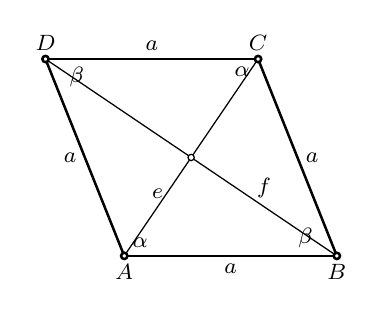
\begin{tikzpicture}
                    % \clip (0,0) rectangle (14.000000,10.000000);
                    {\footnotesize

                    % Marking point a
                    \draw (3.850000,1.500000) node [anchor=north] { $a$ };%

                    % Marking point a
                    \draw (2.850000,4.000000) node [anchor=south] { $a$ };%

                    % Marking point a
                    \draw (4.700000,2.750000) node [anchor=west] { $a$ };%

                    % Marking point a
                    \draw (2.000000,2.750000) node [anchor=east] { $a$ };%

                    % Drawing segment A C
                    \draw [line width=0.016cm] (2.522492,1.533077) -- (3.327508,2.716923);%
                    \draw [line width=0.016cm] (3.372492,2.783077) -- (4.177508,3.966923);%

                    % Drawing segment B D
                    \draw [line width=0.016cm] (5.166856,1.522394) -- (3.383144,2.727606);%
                    \draw [line width=0.016cm] (3.316856,2.772394) -- (1.533144,3.977606);%

                    % Marking point S by circle
                    \draw [line width=0.016cm] (3.350000,2.750000) circle (0.040000);%

                    % Marking point e
                    \draw (2.925000,2.125000) node [anchor=south] { $e$ };%

                    % Marking point f
                    \draw (4.275000,2.125000) node [anchor=south] { $f$ };%

                    % Marking point \alpha
                    \draw (2.500000,1.500000) node [anchor=south west] { $\alpha$ };%

                    % Marking point \beta
                    \draw (5.000000,1.500000) node [anchor=south east] { $\beta$ };%

                    % Marking point \alpha
                    \draw (4.200000,4.000000) node [anchor=north east] { $\alpha$ };%

                    % Marking point \beta
                    \draw (1.700000,4.000000) node [anchor=north west] { $\beta$ };%

                    % Drawing segment A B
                    \draw [line width=0.032cm] (2.540000,1.500000) -- (5.160000,1.500000);%

                    % Drawing segment B C
                    \draw [line width=0.032cm] (5.185144,1.537139) -- (4.214856,3.962861);%

                    % Drawing segment C D
                    \draw [line width=0.032cm] (4.160000,4.000000) -- (1.540000,4.000000);%

                    % Drawing segment D A
                    \draw [line width=0.032cm] (1.514856,3.962861) -- (2.485144,1.537139);%

                    % Marking point A by circle
                    \draw [line width=0.032cm] (2.500000,1.500000) circle (0.040000);%
                    \draw (2.500000,1.500000) node [anchor=north] { $A$ };%

                    % Marking point B by circle
                    \draw [line width=0.032cm] (5.200000,1.500000) circle (0.040000);%
                    \draw (5.200000,1.500000) node [anchor=north] { $B$ };%

                    % Marking point C by circle
                    \draw [line width=0.032cm] (4.200000,4.000000) circle (0.040000);%
                    \draw (4.200000,4.000000) node [anchor=south] { $C$ };%

                    % Marking point D by circle
                    \draw [line width=0.032cm] (1.500000,4.000000) circle (0.040000);%
                    \draw (1.500000,4.000000) node [anchor=south] { $D$ };%
                    }
                    \end{tikzpicture}
                \end{figure}
            \end{definicija}

            
                Diagonali v rombu se razpolavljata in razpolavljata notranje kote, sekata se pod pravim kotom.
            
        



        
            \subsection*{Trapez}
            
            \begin{definicija}
                \textbf{Trapez} je štirikotnik, ki ima en par vzporednih stranic.

                Vzporedni stranici imenujemo \textbf{osnovnici} trapeza, preostali dve stranici pa \textbf{kraka} trapeza.
                \begin{figure}[H]
                    \centering
                    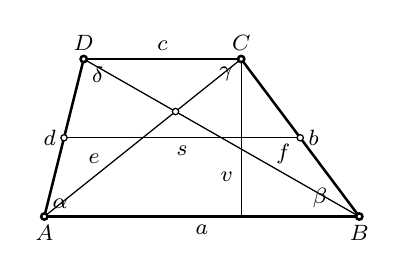
\begin{tikzpicture}
                    % \clip (0,0) rectangle (14.000000,10.000000);
                    {\footnotesize

                    % Marking point a
                    \draw (4.500000,1.500000) node [anchor=north] { $a$ };%

                    % Marking point c
                    \draw (4.000000,3.500000) node [anchor=south] { $c$ };%

                    % Marking point b by circle
                    \draw [line width=0.016cm] (5.750000,2.500000) circle (0.040000);%
                    \draw (5.750000,2.500000) node [anchor=west] { $b$ };%

                    % Marking point d by circle
                    \draw [line width=0.016cm] (2.750000,2.500000) circle (0.040000);%
                    \draw (2.750000,2.500000) node [anchor=east] { $d$ };%

                    % Drawing segment b d
                    \draw [line width=0.016cm] (5.710000,2.500000) -- (2.790000,2.500000);%

                    % Marking point s
                    \draw (4.250000,2.500000) node [anchor=north] { $s$ };%

                    % Drawing segment A C
                    \draw [line width=0.016cm] (2.531235,1.524988) -- (4.135432,2.808346);%
                    \draw [line width=0.016cm] (4.197901,2.858321) -- (4.968765,3.475012);%

                    % Drawing segment B D
                    \draw [line width=0.016cm] (6.465270,1.519846) -- (4.201396,2.813488);%
                    \draw [line width=0.016cm] (4.131937,2.853179) -- (3.034730,3.480154);%

                    % Marking point S by circle
                    \draw [line width=0.016cm] (4.166667,2.833333) circle (0.040000);%

                    % Marking point e
                    \draw (3.133333,2.066667) node [anchor=south] { $e$ };%

                    % Marking point f
                    \draw (5.533333,2.066667) node [anchor=south] { $f$ };%

                    % Marking point \alpha
                    \draw (2.500000,1.500000) node [anchor=south west] { $\alpha$ };%

                    % Marking point \beta
                    \draw (6.200000,1.500000) node [anchor=south east] { $\beta$ };%

                    % Marking point \gamma
                    \draw (5.000000,3.500000) node [anchor=north east] { $\gamma$ };%

                    % Marking point \delta
                    \draw (3.000000,3.500000) node [anchor=north west] { $\delta$ };%

                    % Drawing segment C N
                    \draw [line width=0.016cm] (5.000000,3.460000) -- (5.000000,1.500000);%

                    % Marking point v
                    \draw (5.000000,2.000000) node [anchor=east] { $v$ };%

                    % Drawing segment A B
                    \draw [line width=0.032cm] (2.540000,1.500000) -- (6.460000,1.500000);%

                    % Drawing segment B C
                    \draw [line width=0.032cm] (6.476000,1.532000) -- (5.774000,2.468000);%
                    \draw [line width=0.032cm] (5.726000,2.532000) -- (5.024000,3.468000);%

                    % Drawing segment C D
                    \draw [line width=0.032cm] (4.960000,3.500000) -- (3.040000,3.500000);%

                    % Drawing segment D A
                    \draw [line width=0.032cm] (2.990299,3.461194) -- (2.759701,2.538806);%
                    \draw [line width=0.032cm] (2.740299,2.461194) -- (2.509701,1.538806);%

                    % Marking point A by circle
                    \draw [line width=0.032cm] (2.500000,1.500000) circle (0.040000);%
                    \draw (2.500000,1.500000) node [anchor=north] { $A$ };%

                    % Marking point B by circle
                    \draw [line width=0.032cm] (6.500000,1.500000) circle (0.040000);%
                    \draw (6.500000,1.500000) node [anchor=north] { $B$ };%

                    % Marking point C by circle
                    \draw [line width=0.032cm] (5.000000,3.500000) circle (0.040000);%
                    \draw (5.000000,3.500000) node [anchor=south] { $C$ };%

                    % Marking point D by circle
                    \draw [line width=0.032cm] (3.000000,3.500000) circle (0.040000);%
                    \draw (3.000000,3.500000) node [anchor=south] { $D$ };%
                    }
                    \end{tikzpicture}
                \end{figure}

            \end{definicija}

            \begin{definicija}
                \textbf{Srednica} trapeza je daljica, ki povezuje razpolovišči krakov trapeza.
            \end{definicija}

            \begin{izrek}
                Srednica je vzporedna je osnovnicama, njena dolžina je enaka aritmetični sredini dolžin obeh osnovnic:
                $$s=\frac{a+c}{2}.$$
            \end{izrek}

            
                Višina trapeza je razdalja med osnovnicama.
            

            \begin{trditev}
                Kota ob istem kraku sta suplementarna ($\alpha+\delta=180^\circ$ in $\beta+\gamma=180^\circ$).
            \end{trditev}
        

        
            \begin{definicija}
                \textbf{Enakokraki trapez} je trapez, katerega kraka sta skladna.

                \begin{figure}[H]
                    \centering
                    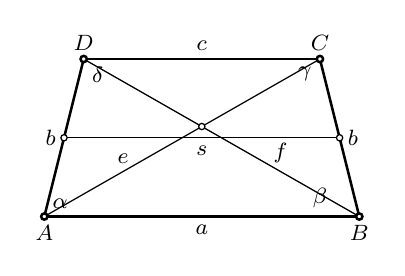
\begin{tikzpicture}
                    % \clip (0,0) rectangle (14.000000,10.000000);
                    {\footnotesize

                    % Marking point a
                    \draw (4.500000,1.500000) node [anchor=north] { $a$ };%

                    % Marking point c
                    \draw (4.500000,3.500000) node [anchor=south] { $c$ };%

                    % Marking point b by circle
                    \draw [line width=0.016cm] (6.250000,2.500000) circle (0.040000);%
                    \draw (6.250000,2.500000) node [anchor=west] { $b$ };%

                    % Marking point d by circle
                    \draw [line width=0.016cm] (2.750000,2.500000) circle (0.040000);%
                    \draw (2.750000,2.500000) node [anchor=east] { $b$ };%

                    % Drawing segment b d
                    \draw [line width=0.016cm] (6.210000,2.500000) -- (2.790000,2.500000);%

                    % Marking point s
                    \draw (4.500000,2.500000) node [anchor=north] { $s$ };%

                    % Drawing segment A C
                    \draw [line width=0.016cm] (2.534730,1.519846) -- (4.465270,2.623012);%
                    \draw [line width=0.016cm] (4.534730,2.662703) -- (5.965270,3.480154);%

                    % Drawing segment B D
                    \draw [line width=0.016cm] (6.465270,1.519846) -- (4.534730,2.623012);%
                    \draw [line width=0.016cm] (4.465270,2.662703) -- (3.034730,3.480154);%

                    % Marking point S by circle
                    \draw [line width=0.016cm] (4.500000,2.642857) circle (0.040000);%

                    % Marking point e
                    \draw (3.500000,2.071429) node [anchor=south] { $e$ };%

                    % Marking point f
                    \draw (5.500000,2.071429) node [anchor=south] { $f$ };%

                    % Marking point \alpha
                    \draw (2.500000,1.500000) node [anchor=south west] { $\alpha$ };%

                    % Marking point \beta
                    \draw (6.200000,1.500000) node [anchor=south east] { $\beta$ };%

                    % Marking point \gamma
                    \draw (6.000000,3.500000) node [anchor=north east] { $\gamma$ };%

                    % Marking point \delta
                    \draw (3.000000,3.500000) node [anchor=north west] { $\delta$ };%

                    % Drawing segment A B
                    \draw [line width=0.032cm] (2.540000,1.500000) -- (6.460000,1.500000);%

                    % Drawing segment B C
                    \draw [line width=0.032cm] (6.490299,1.538806) -- (6.259701,2.461194);%
                    \draw [line width=0.032cm] (6.240299,2.538806) -- (6.009701,3.461194);%

                    % Drawing segment C D
                    \draw [line width=0.032cm] (5.960000,3.500000) -- (3.040000,3.500000);%

                    % Drawing segment D A
                    \draw [line width=0.032cm] (2.990299,3.461194) -- (2.759701,2.538806);%
                    \draw [line width=0.032cm] (2.740299,2.461194) -- (2.509701,1.538806);%

                    % Marking point A by circle
                    \draw [line width=0.032cm] (2.500000,1.500000) circle (0.040000);%
                    \draw (2.500000,1.500000) node [anchor=north] { $A$ };%

                    % Marking point B by circle
                    \draw [line width=0.032cm] (6.500000,1.500000) circle (0.040000);%
                    \draw (6.500000,1.500000) node [anchor=north] { $B$ };%

                    % Marking point C by circle
                    \draw [line width=0.032cm] (6.000000,3.500000) circle (0.040000);%
                    \draw (6.000000,3.500000) node [anchor=south] { $C$ };%

                    % Marking point D by circle
                    \draw [line width=0.032cm] (3.000000,3.500000) circle (0.040000);%
                    \draw (3.000000,3.500000) node [anchor=south] { $D$ };%
                    }
                    \end{tikzpicture}
                \end{figure}
            \end{definicija}

            
                Enakokraki trapez ima skladni diagonali ($e=f$) in skladna para kotov ob isti osnovnici ($\alpha=\beta$ in $\gamma=\delta$).
            
            
        

        

        
            \subsection*{Trapezoid}
            
            \begin{definicija}
                \textbf{Deltoid} je štirikotnik, ki ima dva para sosednjih skladnih nevzporednih stranic.         
                
                \begin{figure}[H]
                    \centering
                    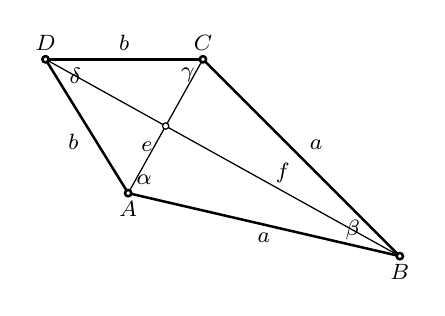
\begin{tikzpicture}
                    % \clip (0,0) rectangle (14.000000,10.000000);
                    {\footnotesize

                    % Marking point a
                    \draw (4.275000,1.900000) node [anchor=north] { $a$ };%

                    % Marking point b
                    \draw (2.500000,4.000000) node [anchor=south] { $b$ };%

                    % Marking point a
                    \draw (4.750000,2.750000) node [anchor=south west] { $a$ };%

                    % Marking point b
                    \draw (2.025000,3.150000) node [anchor=north east] { $b$ };%

                    % Drawing segment A C
                    \draw [line width=0.016cm] (2.569513,2.334918) -- (3.006672,3.117202);%
                    \draw [line width=0.016cm] (3.045697,3.187037) -- (3.480487,3.965082);%

                    % Drawing segment B D
                    \draw [line width=0.016cm] (5.965034,1.519426) -- (3.061151,3.132694);%
                    \draw [line width=0.016cm] (2.991218,3.171545) -- (1.534966,3.980574);%

                    % Marking point S by circle
                    \draw [line width=0.016cm] (3.026185,3.152120) circle (0.040000);%

                    % Marking point e
                    \draw (2.788092,2.726060) node [anchor=south] { $e$ };%

                    % Marking point f
                    \draw (4.513092,2.326060) node [anchor=south] { $f$ };%

                    % Marking point \alpha
                    \draw (2.550000,2.300000) node [anchor=south west] { $\alpha$ };%

                    % Marking point \beta
                    \draw (5.600000,1.600000) node [anchor=south east] { $\beta$ };%

                    % Marking point \gamma
                    \draw (3.500000,4.000000) node [anchor=north east] { $\gamma$ };%

                    % Marking point \delta
                    \draw (1.700000,4.000000) node [anchor=north west] { $\delta$ };%

                    % Drawing segment A B
                    \draw [line width=0.032cm] (2.588966,2.290964) -- (5.961034,1.509036);%

                    % Drawing segment B C
                    \draw [line width=0.032cm] (5.971716,1.528284) -- (3.528284,3.971716);%

                    % Drawing segment C D
                    \draw [line width=0.032cm] (3.460000,4.000000) -- (1.540000,4.000000);%

                    % Drawing segment D A
                    \draw [line width=0.032cm] (1.521020,3.965968) -- (2.528980,2.334032);%

                    % Marking point A by circle
                    \draw [line width=0.032cm] (2.550000,2.300000) circle (0.040000);%
                    \draw (2.550000,2.300000) node [anchor=north] { $A$ };%

                    % Marking point B by circle
                    \draw [line width=0.032cm] (6.000000,1.500000) circle (0.040000);%
                    \draw (6.000000,1.500000) node [anchor=north] { $B$ };%

                    % Marking point C by circle
                    \draw [line width=0.032cm] (3.500000,4.000000) circle (0.040000);%
                    \draw (3.500000,4.000000) node [anchor=south] { $C$ };%

                    % Marking point D by circle
                    \draw [line width=0.032cm] (1.500000,4.000000) circle (0.040000);%
                    \draw (1.500000,4.000000) node [anchor=south] { $D$ };%
                    }
                    \end{tikzpicture}
                \end{figure}
            \end{definicija}

            
                Diagonali deltoida se sekata pod pravim kotom. 
                Daljša diagonala razpolavlja krajšo in oba notranja kota. 
                Preostala kota sta skladna.
            
        


        
            \begin{definicija}
                \textbf{Tetivni štirikotnik} je štirikotnik, katerega stranice so tetive neke krožnice.

                \begin{figure}[H]
                    \centering
                    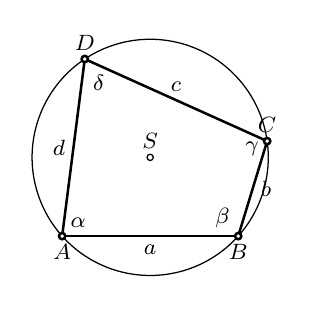
\begin{tikzpicture}
                    % \clip (0,0) rectangle (14.000000,10.000000);
                    {\footnotesize

                    % Marking point a
                    \draw (3.500000,2.000000) node [anchor=north] { $a$ };%

                    % Marking point b
                    \draw (4.801881,2.603211) node [anchor=west] { $b$ };%

                    % Marking point c
                    \draw (3.827443,3.727651) node [anchor=south] { $c$ };%

                    % Marking point d
                    \draw (2.525561,3.124440) node [anchor=east] { $d$ };%

                    % Marking point \alpha
                    \draw (2.381966,2.000000) node [anchor=south west] { $\alpha$ };%

                    % Marking point \beta
                    \draw (4.618034,2.000000) node [anchor=south east] { $\beta$ };%

                    % Marking point \gamma
                    \draw (4.985729,3.306422) node [anchor=north east] { $\gamma$ };%

                    % Marking point \delta
                    \draw (2.669157,4.148879) node [anchor=north west] { $\delta$ };%

                    % Drawing circle k
                    \draw [line width=0.016cm] (5.000000,3.000000) arc (360:360:1.500000 and 1.500000) --(5.000000,3.000000) arc (0:6:1.500000 and 1.500000) -- (4.990705,3.166733);%
                    \draw [line width=0.016cm] (4.979696,3.245965) -- (4.977212,3.260472) arc (10:122:1.500000 and 1.500000) -- (2.702753,4.270589);%
                    \draw [line width=0.016cm] (2.636152,4.226282) -- (2.618322,4.213526) arc (126:220:1.500000 and 1.500000) -- (2.355699,2.030167);%
                    \draw [line width=0.016cm] (2.409028,1.970544) -- (2.420990,1.958013) arc (224:316:1.500000 and 1.500000) -- (4.590972,1.970544);%
                    \draw [line width=0.016cm] (4.644300,2.030167) -- (4.649066,2.035818) arc (320:360:1.500000 and 1.500000);%

                    % Marking point S by circle
                    \draw [line width=0.016cm] (3.500000,3.000000) circle (0.040000);%
                    \draw (3.500000,3.000000) node [anchor=south] { $S$ };%

                    % Drawing segment A B
                    \draw [line width=0.032cm] (2.421966,2.000000) -- (4.578034,2.000000);%

                    % Drawing segment B C
                    \draw [line width=0.032cm] (4.629696,2.038262) -- (4.974067,3.168160);%

                    % Drawing segment C D
                    \draw [line width=0.032cm] (4.949252,3.222837) -- (2.705634,4.232465);%

                    % Drawing segment D A
                    \draw [line width=0.032cm] (2.664090,4.209202) -- (2.387033,2.039678);%

                    % Marking point A by circle
                    \draw [line width=0.032cm] (2.381966,2.000000) circle (0.040000);%
                    \draw (2.381966,2.000000) node [anchor=north] { $A$ };%

                    % Marking point B by circle
                    \draw [line width=0.032cm] (4.618034,2.000000) circle (0.040000);%
                    \draw (4.618034,2.000000) node [anchor=north] { $B$ };%

                    % Marking point C by circle
                    \draw [line width=0.032cm] (4.985729,3.206422) circle (0.040000);%
                    \draw (4.985729,3.206422) node [anchor=south] { $C$ };%

                    % Marking point D by circle
                    \draw [line width=0.032cm] (2.669157,4.248879) circle (0.040000);%
                    \draw (2.669157,4.248879) node [anchor=south] { $D$ };%
                    }
                    \end{tikzpicture}
                \end{figure}
            \end{definicija}

            \begin{izrek}
                Nasprotna kota tetivnega štirikotnika sta suplementarna:
                
                $$\alpha+\gamma=\beta+\delta=180^\circ.$$
            \end{izrek}

            \begin{trditev}
                Če sta v štirikotniku nasprotna kota suplementarna, mu lahko očrtamo krožnico.
            \end{trditev}
        


        
            \begin{definicija}
                \textbf{Tangentni štirikotnik} je štirikotnik, katerega stranice so odseki na tangentah neke krožnice.

                \begin{figure}[H]
                    \centering
                    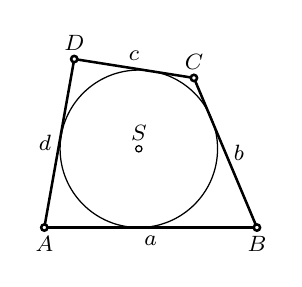
\begin{tikzpicture}
                    % \clip (0,0) rectangle (14.000000,10.000000);
                    {\footnotesize

                    % Marking point a
                    \draw (3.650000,1.500000) node [anchor=north] { $a$ };%

                    % Marking point b
                    \draw (4.600000,2.450000) node [anchor=west] { $b$ };%

                    % Marking point c
                    \draw (3.440000,3.520000) node [anchor=south] { $c$ };%

                    % Marking point d
                    \draw (2.490000,2.570000) node [anchor=east] { $d$ };%

                    % % Marking point \alpha
                    % \draw (2.300000,1.500000) node [anchor=south west] { $\alpha$ };%

                    % % Marking point \beta
                    % \draw (5.000000,1.500000) node [anchor=south east] { $\beta$ };%

                    % % Marking point \gamma
                    % \draw (4.200000,3.400000) node [anchor=north east] { $\gamma$ };%

                    % % Marking point \delta
                    % \draw (2.680000,3.640000) node [anchor=north west] { $\delta$ };%

                    % Drawing circle k
                    \draw [line width=0.016cm] (3.500000,2.500000) circle (1.000000);%

                    % Marking point S by circle
                    \draw [line width=0.016cm] (3.500000,2.500000) circle (0.040000);%
                    \draw (3.500000,2.500000) node [anchor=south] { $S$ };%

                    % Drawing segment A B
                    \draw [line width=0.032cm] (2.340000,1.500000) -- (4.960000,1.500000);%

                    % Drawing segment B C
                    \draw [line width=0.032cm] (4.984478,1.536865) -- (4.215522,3.363135);%

                    % Drawing segment C D
                    \draw [line width=0.032cm] (4.160489,3.406239) -- (2.719511,3.633761);%

                    % Drawing segment D A
                    \draw [line width=0.032cm] (2.673007,3.600616) -- (2.306993,1.539384);%

                    % Marking point A by circle
                    \draw [line width=0.032cm] (2.300000,1.500000) circle (0.040000);%
                    \draw (2.300000,1.500000) node [anchor=north] { $A$ };%

                    % Marking point B by circle
                    \draw [line width=0.032cm] (5.000000,1.500000) circle (0.040000);%
                    \draw (5.000000,1.500000) node [anchor=north] { $B$ };%

                    % Marking point C by circle
                    \draw [line width=0.032cm] (4.200000,3.400000) circle (0.040000);%
                    \draw (4.200000,3.400000) node [anchor=south] { $C$ };%

                    % Marking point D by circle
                    \draw [line width=0.032cm] (2.680000,3.640000) circle (0.040000);%
                    \draw (2.680000,3.640000) node [anchor=south] { $D$ };%
                    }
                    \end{tikzpicture}
                \end{figure}
            \end{definicija}

            \begin{izrek}
                Vsota dolžin nasprotnih stranic tangentnega štirikotnika je enaka vsoti dolžin drugih dveh nasprotnih stranic:
                
                $$a+c=b+d.$$
            \end{izrek}
        


        
            \subsection*{Pravilni $n$-kotnik}

            \begin{definicija}
                \textbf{Pravlni $n$-kotnik} ima vse stranice enako dolge in vse kote enako velike.

                \begin{figure}[H]
                    \centering

                \end{figure}
            \end{definicija}

            \begin{izrek}
                Vsota notranjih kotov trikotnika je $(n-2)\cdot 180^\circ$.
            \end{izrek}

            
                Notranji kot pravilnega $n$-kotnika meri $\frac{n-2}{n} 180^\circ$.
            

        


        
            \begin{naloga}
                Konstruirajte paralelogram $ABCD$ s podatki:
                \begin{itemize}
                    \item $a=4~cm$, $b=3~cm$, $e=6~cm$;
                    \item $\alpha=60^\circ$, $a=5~cm$, $b=3~cm$;
                    \item $e=f=4~cm$, $a=3~cm$.
                \end{itemize}
            \end{naloga}

            \begin{naloga}
                Konstruirajte trapez $ABCD$ s podatki:
                \begin{itemize}
                    \item $a=5~cm$, $b=4~cm$, $d=3.5~cm$, $\beta=60^\circ$;
                    \item $a=4~cm$, $v=3~cm$, $e=5~cm$, $f=4~cm$;
                    \item $\alpha=60^\circ$, $a=5~cm$, $e=f=4.5~cm$;
                    \item $\alpha=60^\circ$, $b=5~cm$, $c=2~cm$, $v=4~cm$.
                \end{itemize}
            \end{naloga}

        


        
            \begin{naloga}
                Konstruirajte deltoid $ABCD$ s podatki:
                \begin{itemize}
                    \item $b=3.5~cm$, $e=4~cm$, $f=5~cm$;
                    \item $a=4~cm$, $b=3~cm$, $\delta=90^\circ$.
                \end{itemize}
            \end{naloga}

            \begin{naloga}
                
            \end{naloga}
        